\documentclass[11pt]{article}

\usepackage[margin=1in]{geometry}
\usepackage[T1]{fontenc}
\usepackage[utf8]{inputenc}
\usepackage{lmodern}
\usepackage{microtype}
\usepackage{amsmath,amssymb}
\usepackage{booktabs}
\usepackage{graphicx}
\usepackage{float}
\usepackage{pdflscape}
\usepackage{threeparttable}
\usepackage{siunitx}
\usepackage{caption}
\usepackage[hidelinks]{hyperref}
\usepackage{xcolor}

\graphicspath{{outputs/figures/}}
\captionsetup{font=small,labelfont=bf}
\sisetup{
  detect-all,
  group-separator={,},
  group-minimum-digits=4,
  exponent-product=\times,
  output-exponent-marker=\mathrm{e}
}
\newcommand{\NA}{\multicolumn{1}{c}{--}}
\newcommand{\E}{\mathbb{E}}
\newcommand{\Var}{\operatorname{Var}}
\newcommand{\Corr}{\operatorname{Corr}}

\title{\textbf{Liquidity, Price Dynamics, and Triangular Arbitrage}\\
\large Evidence from NASDAQ and Foreign-Exchange Limit Order Books}
\author{Alexandre Marthan \and Elias Roubache \and Jean Jacob \and Matthieu Pascal \and Elouan Bahri}
\date{MFE 230X --- High-Frequency Finance, Fall 2026}

\begin{document}
\maketitle

\begin{abstract}
This report studies one trading session for two NASDAQ stocks and the assigned EUR/USD--USD/JPY--EUR/JPY currency triangle. AAPL and GPRO were selected to expose the same measurement pipeline to two very different market structures: an actively traded large-cap stock and a thin, low-priced stock whose quoted spread is constrained by the one-cent tick. AAPL trades roughly \$4.42 million per minute, compared with only \$9.66 thousand for GPRO. The liquidity ranking is correspondingly sharp: mean five-second price impact is 0.56 basis points for AAPL and 13.25 basis points for GPRO. In foreign exchange, the main intraday event is the London close rather than the New York equity open. We also identify 28 one-second triangular-arbitrage observations grouped into 20 episodes. Their frictionless marked profit is economically small and remains an upper bound because the data do not include fees, last-look rejections, or execution latency. The follow-up instruction requests Monday--Friday liquidity plots; the present report is explicitly a one-day cross-sectional case study, and the weekly extension and its testable implications are stated below.
\end{abstract}

\section{Introduction}

The objective is to characterize trading activity, liquidity, short-horizon price dynamics, and executable triangular arbitrage using high-frequency order-book and transaction data. The equity sample contains AAPL and GPRO on 30 December 2019 from 09:30 to 16:00 Eastern Time. AAPL is a large-cap, high-turnover stock. GPRO is a small-cap stock trading near \$4.34, so its one-cent minimum tick is economically large. The comparison is therefore not a universe-wide stock-selection exercise. It is a controlled contrast between a thick, continuously refreshed book and a sparse, tick-constrained book processed with the same code.

The economic prior follows the information-asymmetry logic of Glosten and Milgrom \cite{glosten1985} and Kyle \cite{kyle1985}. When a dealer has less uninformed order flow against which to average informed trading, adverse-selection costs should appear in wider relative spreads and greater price impact. The AAPL--GPRO comparison is consistent with that prediction, but the intraday evidence requires more care: GPRO's spread is primarily a tick-size outcome, not a smooth information-driven U-shape.

The currency sample contains EUR/USD, USD/JPY, and EUR/JPY on 25 January 2012 over the same 09:30--16:00 clock. These pairs are prescribed by the assignment and form a closed conversion triangle. Because this interval overlaps both London and New York trading, foreign-exchange results should not be forced into a U.S.-equity opening narrative.

The main findings are:
\begin{itemize}
  \item AAPL trades approximately 457 times more dollar volume per minute than GPRO. GPRO appears deeper in shares at the best bid, but AAPL is deeper in dollar terms.
  \item AAPL's spread and price impact are elevated at the open and then decline; its close does not recreate the second arm of a textbook U-shape on this holiday-week Monday.
  \item GPRO's one-cent spread binds nearly all day. Its 14:30 variance spike is a sparse-trading burst, not a simultaneous spread widening or depth collapse.
  \item The three currency pairs experience a synchronized spread and variance event around the London close. EUR/JPY is the widest and sparsest leg and exhibits the clearest one-minute reversal.
  \item Apparent triangular arbitrage is rare, brief, and small after accounting for realistic implementation limits.
\end{itemize}

\section{Data and Measurement}

\subsection{Data construction}

NASDAQ trades and ten-level market-by-price books are obtained from Databento. Market-by-order records supply new-order counts. Timestamps are converted from UTC to New York time and processed in exchange-event time. A ten-minute pre-open buffer seeds the 09:30 stock book. Currency books are reconstructed from the two supplied EBS files, using integer price ticks as book keys and treating each size update as a replacement of the quantity at that price.

Stock dollar volume is price times shares. Currency volume is converted to U.S. dollars: EUR/USD is already in dollar notional, USD/JPY size is in dollars, and EUR/JPY yen notional is divided by the same-second USD/JPY midpoint. Equity order counts include genuine displayed additions and exclude replacement-generated add messages. Hidden trades remain in transaction-based volume and price measures but cannot be counted as displayed new orders.

\subsection{Scope relative to the five-day requirement}
\label{sec:week}

The assignment follow-up asks for the three liquidity measures---spread, depth, and price impact---to be plotted and compared over five consecutive trading days from Monday through Friday. The locked submission contains one NASDAQ session and one currency session. We therefore do not present the current figures as a completed weekly comparison. The narrower design deliberately emphasizes the cross section: how the same estimators behave for AAPL versus GPRO and across the three legs of the currency triangle, rather than how one ticker's intraday profile changes from day to day. This focus permits a detailed treatment of the tick constraint, sparse impact identification, dollar versus share depth, and market-specific event clocks, but it cannot identify persistent day-of-week patterns.

\paragraph{Expected results from a full week.}
A five-day extension would first plot each daily profile separately and then compare a cross-day mean profile with day-level dispersion bands. If the equity patterns are structural, AAPL should repeatedly open with wider spreads, higher impact, and greater variance; a less holiday-affected week may also restore the usual late-day rise that is absent on 30 December 2019. GPRO's one-cent spread should remain comparatively flat whenever the tick binds, while isolated variance bursts such as the 14:30 event should move across days or disappear if they are idiosyncratic. Repetition would distinguish a stable thin-name pattern from a single-day print. In foreign exchange, recurring spread and impact widening near the London close would support the event-clock interpretation; failure to recur would recast the 12:25 move as date-specific. Pooling five days would also provide more identified impact minutes for the sparse instruments, tighter uncertainty around intraday averages, and a more reliable estimate of triangular-arbitrage frequency and duration. These are predictions for the unobserved weekly panel, not results inferred from the one-day sample.

\subsection{Liquidity measures}

Let $a_t$ and $b_t$ denote the best ask and bid. The quoted spread is
\begin{equation}
  s_t=a_t-b_t.
\end{equation}
Because quotes are piecewise constant, spread and depth are averaged by the duration for which each book state is valid:
\begin{equation}
  \bar{s}_{\Delta}
  =\frac{\sum_i s_i\,\Delta t_i}{\sum_i \Delta t_i}.
\end{equation}
Figures report the spread in basis points of the corresponding five-minute VWAP,
\begin{equation}
  s_{\Delta}^{\mathrm{bps}}
  =10^4\frac{\bar{s}_{\Delta}}{\mathrm{VWAP}_{\Delta}}.
\end{equation}

Level-one depth is the displayed quantity at the best bid and ask, reported separately. Depth at twice the daily average spread sums all displayed bid quantities at prices above $m_t-2\bar{s}_{\mathrm{day}}$ and all ask quantities below $m_t+2\bar{s}_{\mathrm{day}}$, where $m_t=(a_t+b_t)/2$. Following the assignment convention, both band-depth measures are zero when the contemporaneous spread exceeds twice its daily time-weighted average. Stock band depth is limited to the ten observed levels; the diagnostics confirm that this limit does not truncate the band in the present sample.

Five-second price impact is estimated separately in each minute:
\begin{equation}
  \frac{m_{t+5}-m_t}{m_t}
  =\alpha_{\tau}+\lambda_{\tau}\,\mathrm{sign}_t+\varepsilon_t,
  \qquad \mathrm{sign}_t\in\{-1,+1\}.
\end{equation}
A minute is retained only when it contains at least five signed trades and both trade directions. This rule gives stable identification for AAPL and EUR/USD but leaves many missing estimates for GPRO and EUR/JPY. Reported impact means therefore refer only to identified minutes.

\subsection{Prices, returns, and dependence}

The last midpoint and transaction price in each one-second and one-minute interval are retained. After the first valid observation, the last price is carried forward through an empty interval. Log returns are
\begin{equation}
  r_t=\log p_t-\log p_{t-1},
\end{equation}
and realized variance is $\sum_t r_t^2$. Autocorrelations are calculated through lag 10; lag 0, which equals one by construction, is omitted from the plot. Thirty-minute variance and lag-1 autocorrelation use the one-minute transaction-return series. An opening half-hour contains 29 returns; subsequent bins contain 30.

\subsection{Triangular arbitrage}

The one-second currency books are synchronized and required to be strictly positive and uncrossed. Two aggressive conversion loops are tested:
\begin{align}
  L_A &= \frac{b_{\mathrm{EUR/USD}}\,b_{\mathrm{USD/JPY}}}
               {a_{\mathrm{EUR/JPY}}},\\
  L_B &= \frac{b_{\mathrm{EUR/JPY}}}
               {a_{\mathrm{USD/JPY}}\,a_{\mathrm{EUR/USD}}}.
\end{align}
An opportunity exists when either loop exceeds one. Every leg crosses the spread: purchases execute at the ask and sales at the bid. Tradable quantity is the minimum BBO capacity across the three legs after conversion to euros. Marked profit is frictionless and therefore excludes fees, last look, communication delay, and partial fills.

\section{Summary Statistics}

Tables \ref{tab:activity}--\ref{tab:fx-liquidity} report the number of available minute observations, mean, standard deviation, minimum, 25th percentile, median, 75th percentile, and maximum. Monetary and depth variables are scaled before display so that economically meaningful differences are visible without raw machine notation.

\begin{table}[H]
\centering
\caption{Trading activity per minute}
\label{tab:activity}
\scriptsize
\begin{threeparttable}
\begin{tabular}{@{}llrrrrrrrr@{}}
\toprule
Instrument & Measure & $N$ & Mean & Std. dev. & Min. & P25 & Median & P75 & Max.\\
\midrule
\multicolumn{10}{l}{\textit{Panel A: NASDAQ equities}}\\
AAPL & Dollar volume (\$ millions) & 390 & 4.418 & 5.825 & 0.823 & 2.195 & 3.224 & 5.082 & 97.175\\
     & Trades & 390 & 171.99 & 123.69 & 50 & 101 & 135.5 & 193.8 & 1,272\\
     & New orders & 390 & 1,780.82 & 1,429.99 & 697 & 1,130.5 & 1,461.5 & 1,968.0 & 23,806\\
GPRO & Dollar volume (\$ millions) & 390 & 0.00966 & 0.02667 & 0 & 0 & 0.00043 & 0.00739 & 0.33232\\
     & Trades & 390 & 7.22 & 13.90 & 0 & 0 & 2 & 7.8 & 143\\
     & New orders & 390 & 68.30 & 135.83 & 2 & 17 & 32 & 87.8 & 2,171\\
\addlinespace
\multicolumn{10}{l}{\textit{Panel B: Foreign exchange}}\\
EUR/USD & Dollar volume (\$ millions) & 390 & 105.613 & 144.871 & 0 & 35.013 & 64.851 & 113.909 & 1,818.583\\
        & Trades & 390 & 37.27 & 36.64 & 0 & 16 & 27 & 42 & 340\\
USD/JPY & Dollar volume (\$ millions) & 390 & 32.674 & 45.064 & 0 & 8.000 & 19.000 & 40.000 & 413.000\\
        & Trades & 390 & 15.49 & 16.85 & 0 & 5 & 11 & 20 & 155\\
EUR/JPY & Dollar volume (\$ millions) & 390 & 8.002 & 11.676 & 0 & 1.297 & 3.893 & 10.371 & 89.013\\
        & Trades & 390 & 3.95 & 4.95 & 0 & 1 & 2 & 5 & 37\\
\bottomrule
\end{tabular}
\begin{tablenotes}[flushleft]\footnotesize
\item \textit{Notes:} Dollar volume is transaction price times executed quantity and is shown in millions of U.S. dollars per minute. Foreign-exchange orders are not reported because the assignment requests order counts only for NASDAQ ITCH. Zero-volume minutes are retained.
\end{tablenotes}
\end{threeparttable}
\end{table}

The activity contrast motivates the stock selection. AAPL averages \$4.42 million and 172 trades per minute, while GPRO averages only \$9.66 thousand and seven trades. GPRO's median minute contains two trades, and its 25th percentile is zero; AAPL's least active minute still contains 50 trades. EUR/USD is the most active currency pair, followed by USD/JPY and then EUR/JPY.

\begin{landscape}
\begin{table}[H]
\centering
\caption{Minute-level transaction prices}
\label{tab:prices}
\scriptsize
\begin{threeparttable}
\begin{tabular}{@{}llrrrrrrrr@{}}
\toprule
Instrument & Price measure & $N$ & Mean & Std. dev. & Min. & P25 & Median & P75 & Max.\\
\midrule
\multicolumn{10}{l}{\textit{Panel A: NASDAQ equities (U.S. dollars per share)}}\\
AAPL & Open  & 390 & 290.2103 & 2.0734 & 285.4100 & 288.3525 & 291.3350 & 291.6950 & 292.6000\\
     & Close & 390 & 290.2137 & 2.0746 & 285.3400 & 288.3563 & 291.3450 & 291.6975 & 292.6100\\
     & High  & 390 & 290.3270 & 2.0413 & 285.5400 & 288.5425 & 291.4350 & 291.7800 & 292.6900\\
     & Low   & 390 & 290.0994 & 2.1110 & 285.2300 & 288.2375 & 291.2600 & 291.6200 & 292.5500\\
     & VWAP  & 390 & 290.2168 & 2.0760 & 285.4058 & 288.4042 & 291.3432 & 291.7045 & 292.6158\\
GPRO & Open  & 285 & 4.3359 & 0.0689 & 4.2000 & 4.2850 & 4.3200 & 4.3900 & 4.4650\\
     & Close & 285 & 4.3356 & 0.0693 & 4.2100 & 4.2850 & 4.3200 & 4.3900 & 4.4700\\
     & High  & 285 & 4.3377 & 0.0685 & 4.2100 & 4.2900 & 4.3200 & 4.3900 & 4.4700\\
     & Low   & 285 & 4.3336 & 0.0697 & 4.2000 & 4.2850 & 4.3150 & 4.3900 & 4.4650\\
     & VWAP  & 285 & 4.3356 & 0.0690 & 4.2100 & 4.2850 & 4.3200 & 4.3900 & 4.4699\\
\addlinespace
\multicolumn{10}{l}{\textit{Panel B: Foreign exchange (quote currency per unit of base currency)}}\\
EUR/USD & Open  & 389 & 1.302706 & 0.005592 & 1.294880 & 1.297390 & 1.303290 & 1.308100 & 1.312090\\
        & Close & 389 & 1.302735 & 0.005604 & 1.294900 & 1.297400 & 1.303400 & 1.308120 & 1.312090\\
        & High  & 389 & 1.302942 & 0.005630 & 1.295290 & 1.297500 & 1.303660 & 1.308400 & 1.312090\\
        & Low   & 389 & 1.302530 & 0.005571 & 1.294700 & 1.297200 & 1.302920 & 1.307920 & 1.311800\\
        & VWAP  & 389 & 1.302739 & 0.005602 & 1.294931 & 1.297339 & 1.303268 & 1.308174 & 1.311956\\
USD/JPY & Open  & 377 & 77.9485 & 0.2226 & 77.5700 & 77.7300 & 77.8960 & 78.1730 & 78.2820\\
        & Close & 377 & 77.9471 & 0.2230 & 77.5700 & 77.7300 & 77.8920 & 78.1740 & 78.2870\\
        & High  & 377 & 77.9571 & 0.2202 & 77.5990 & 77.7490 & 77.9070 & 78.1800 & 78.2880\\
        & Low   & 377 & 77.9389 & 0.2254 & 77.5600 & 77.7280 & 77.8710 & 78.1700 & 78.2760\\
        & VWAP  & 377 & 77.9479 & 0.2227 & 77.5808 & 77.7340 & 77.8877 & 78.1725 & 78.2810\\
EUR/JPY & Open  & 307 & 101.5338 & 0.1825 & 101.2000 & 101.4000 & 101.4960 & 101.6755 & 101.9400\\
        & Close & 307 & 101.5348 & 0.1831 & 101.2030 & 101.3985 & 101.5000 & 101.6800 & 101.9400\\
        & High  & 307 & 101.5424 & 0.1828 & 101.2030 & 101.4005 & 101.5000 & 101.6900 & 101.9490\\
        & Low   & 307 & 101.5267 & 0.1835 & 101.2000 & 101.3900 & 101.4930 & 101.6720 & 101.9400\\
        & VWAP  & 307 & 101.5350 & 0.1829 & 101.2001 & 101.4005 & 101.5000 & 101.6791 & 101.9400\\
\bottomrule
\end{tabular}
\begin{tablenotes}[flushleft]\footnotesize
\item \textit{Notes:} Statistics summarize one-minute transaction-based open, close, high, low, and volume-weighted average prices. $N<390$ denotes minutes without a transaction; those observations remain missing rather than being imputed in this table.
\end{tablenotes}
\end{threeparttable}
\end{table}
\end{landscape}

\begin{landscape}
\begin{table}[H]
\centering
\caption{NASDAQ liquidity statistics}
\label{tab:stock-liquidity}
\scriptsize
\begin{threeparttable}
\begin{tabular}{@{}llrrrrrrrr@{}}
\toprule
Instrument & Measure & $N$ & Mean & Std. dev. & Min. & P25 & Median & P75 & Max.\\
\midrule
AAPL & BBO spread (cents) & 390 & 2.6357 & 0.5805 & 1.4646 & 2.2523 & 2.5712 & 2.8756 & 5.3829\\
     & Bid depth (000 shares) & 390 & 0.2482 & 0.1367 & 0.1109 & 0.1867 & 0.2165 & 0.2609 & 1.5324\\
     & Ask depth (000 shares) & 390 & 0.2229 & 0.1157 & 0.1118 & 0.1669 & 0.1970 & 0.2413 & 1.6478\\
     & Bid depth, $2\bar{s}$ (000 shares) & 390 & 1.2890 & 0.5334 & 0.4061 & 1.0022 & 1.1876 & 1.4375 & 5.7259\\
     & Ask depth, $2\bar{s}$ (000 shares) & 390 & 1.3445 & 0.7385 & 0.3857 & 0.9836 & 1.1803 & 1.4761 & 7.5540\\
     & Five-second impact (bps) & 390 & 0.5588 & 0.3640 & -0.6182 & 0.3085 & 0.5306 & 0.7481 & 2.8159\\
\addlinespace
GPRO & BBO spread (cents) & 390 & 1.0049 & 0.0387 & 1.0000 & 1.0000 & 1.0000 & 1.0000 & 1.5272\\
     & Bid depth (000 shares) & 390 & 6.2724 & 5.3185 & 0.1971 & 3.3175 & 4.7893 & 7.2681 & 48.3086\\
     & Ask depth (000 shares) & 390 & 7.4832 & 5.3576 & 0.4980 & 3.6800 & 5.9441 & 9.5724 & 27.2236\\
     & Bid depth, $2\bar{s}$ (000 shares) & 390 & 14.7122 & 7.4023 & 1.8160 & 9.8009 & 13.1622 & 17.9248 & 59.1186\\
     & Ask depth, $2\bar{s}$ (000 shares) & 390 & 14.4058 & 7.0990 & 1.7790 & 9.0795 & 12.9261 & 18.6620 & 40.0157\\
     & Five-second impact (bps) & 51 & 13.2520 & 10.3977 & -1.5549 & 5.7039 & 11.5607 & 20.2828 & 42.2978\\
\bottomrule
\end{tabular}
\begin{tablenotes}[flushleft]\footnotesize
\item \textit{Notes:} BBO values are from the NASDAQ TotalView book, not the protected NBBO. Spread and depth are exact event-time-weighted minute means. The $2\bar{s}$ rows sum displayed quantity inside twice the daily average-spread band and are set to zero when the contemporaneous spread exceeds $2\bar{s}$. Impact is $10^4\widehat{\lambda}_{\tau}$ and is available only in minutes meeting the signed-trade identification rule.
\end{tablenotes}
\end{threeparttable}
\end{table}
\end{landscape}

\begin{landscape}
\begin{table}[H]
\centering
\caption{Foreign-exchange liquidity statistics}
\label{tab:fx-liquidity}
\scriptsize
\begin{threeparttable}
\begin{tabular}{@{}llrrrrrrrr@{}}
\toprule
Instrument & Measure & $N$ & Mean & Std. dev. & Min. & P25 & Median & P75 & Max.\\
\midrule
EUR/USD & BBO spread (pips) & 390 & 1.1334 & 0.1674 & 0.6706 & 1.0164 & 1.1235 & 1.2405 & 1.6425\\
        & Bid depth (millions base) & 390 & 2.0304 & 1.0136 & 1.0067 & 1.5238 & 1.7871 & 2.2530 & 10.5385\\
        & Ask depth (millions base) & 390 & 1.9764 & 0.8159 & 1.0400 & 1.5204 & 1.8240 & 2.2074 & 10.0017\\
        & Bid depth, $2\bar{s}$ (millions base) & 390 & 22.2909 & 7.4099 & 9.6717 & 17.9954 & 21.9975 & 26.1454 & 94.4548\\
        & Ask depth, $2\bar{s}$ (millions base) & 390 & 22.1599 & 14.2849 & 9.8717 & 16.9296 & 20.2950 & 24.0926 & 239.5783\\
        & Five-second impact (bps) & 386 & 0.1964 & 0.1635 & -0.4536 & 0.0978 & 0.1780 & 0.2747 & 1.0021\\
\addlinespace
USD/JPY & BBO spread (pips) & 390 & 0.8007 & 0.1580 & 0.4027 & 0.6884 & 0.7947 & 0.8890 & 1.4418\\
        & Bid depth (millions base) & 390 & 2.0955 & 1.0207 & 1.0000 & 1.4542 & 1.8133 & 2.4013 & 7.5017\\
        & Ask depth (millions base) & 390 & 2.2145 & 1.5091 & 1.0000 & 1.4542 & 1.8375 & 2.3129 & 15.2817\\
        & Bid depth, $2\bar{s}$ (millions base) & 390 & 20.1592 & 6.1154 & 8.9000 & 15.1688 & 19.6667 & 24.7271 & 44.7550\\
        & Ask depth, $2\bar{s}$ (millions base) & 390 & 22.2068 & 12.7433 & 6.0667 & 14.5136 & 20.3136 & 24.7524 & 100.2245\\
        & Five-second impact (bps) & 302 & 0.2248 & 0.3061 & -0.4050 & 0.0841 & 0.1912 & 0.3165 & 4.3045\\
\addlinespace
EUR/JPY & BBO spread (pips) & 390 & 1.8982 & 0.3301 & 0.7552 & 1.7035 & 1.9172 & 2.0892 & 3.3197\\
        & Bid depth (millions base) & 390 & 1.4653 & 0.5523 & 1.0000 & 1.1408 & 1.3067 & 1.5833 & 6.7900\\
        & Ask depth (millions base) & 390 & 1.9656 & 3.5727 & 1.0000 & 1.1642 & 1.3683 & 1.7071 & 48.9283\\
        & Bid depth, $2\bar{s}$ (millions base) & 390 & 16.9464 & 2.8538 & 8.0167 & 14.8579 & 16.8817 & 18.6617 & 30.7417\\
        & Ask depth, $2\bar{s}$ (millions base) & 390 & 18.9312 & 8.9422 & 10.2917 & 14.2763 & 16.9467 & 20.6650 & 90.1317\\
        & Five-second impact (bps) & 103 & 0.4630 & 0.4342 & -0.3606 & 0.1730 & 0.4167 & 0.6614 & 1.9398\\
\bottomrule
\end{tabular}
\begin{tablenotes}[flushleft]\footnotesize
\item \textit{Notes:} One pip is $10^{-4}$ for EUR/USD and $10^{-2}$ for the JPY pairs. Depth is in millions of base currency. EUR/USD, USD/JPY, and EUR/JPY have mean relative spreads of approximately 0.87, 1.03, and 1.87 basis points, respectively. Extreme ask-depth maxima are short-lived resting orders rather than typical book states.
\end{tablenotes}
\end{threeparttable}
\end{table}
\end{landscape}

The stock liquidity table reverses the ranking suggested by raw shares. GPRO displays about 6,272 shares at the bid, versus 248 for AAPL, but multiplying by price gives approximately \$27 thousand for GPRO and \$72 thousand for AAPL. AAPL's $2\bar{s}$ bid depth is 5.19 times L1 and its ask depth is 6.03 times L1. GPRO's corresponding ratios are only 2.35 and 1.93 because its average spread is already the minimum tick. EUR/USD lies at the other extreme: roughly 11 times as much displayed size sits inside the $2\bar{s}$ band as at the touch.

Spread and depth comove negatively in every instrument. The L1 correlations range from $-0.10$ for USD/JPY to $-0.32$ for EUR/JPY, while the nearby-book correlations are more negative, reaching $-0.47$ for EUR/JPY. Thus, a wider quote tends to coincide with less displayed quantity nearby, although the relation is not deterministic at the best price alone.

\section{Intraday Liquidity}

\subsection{NASDAQ equities}

\begin{figure}[H]
  \centering
  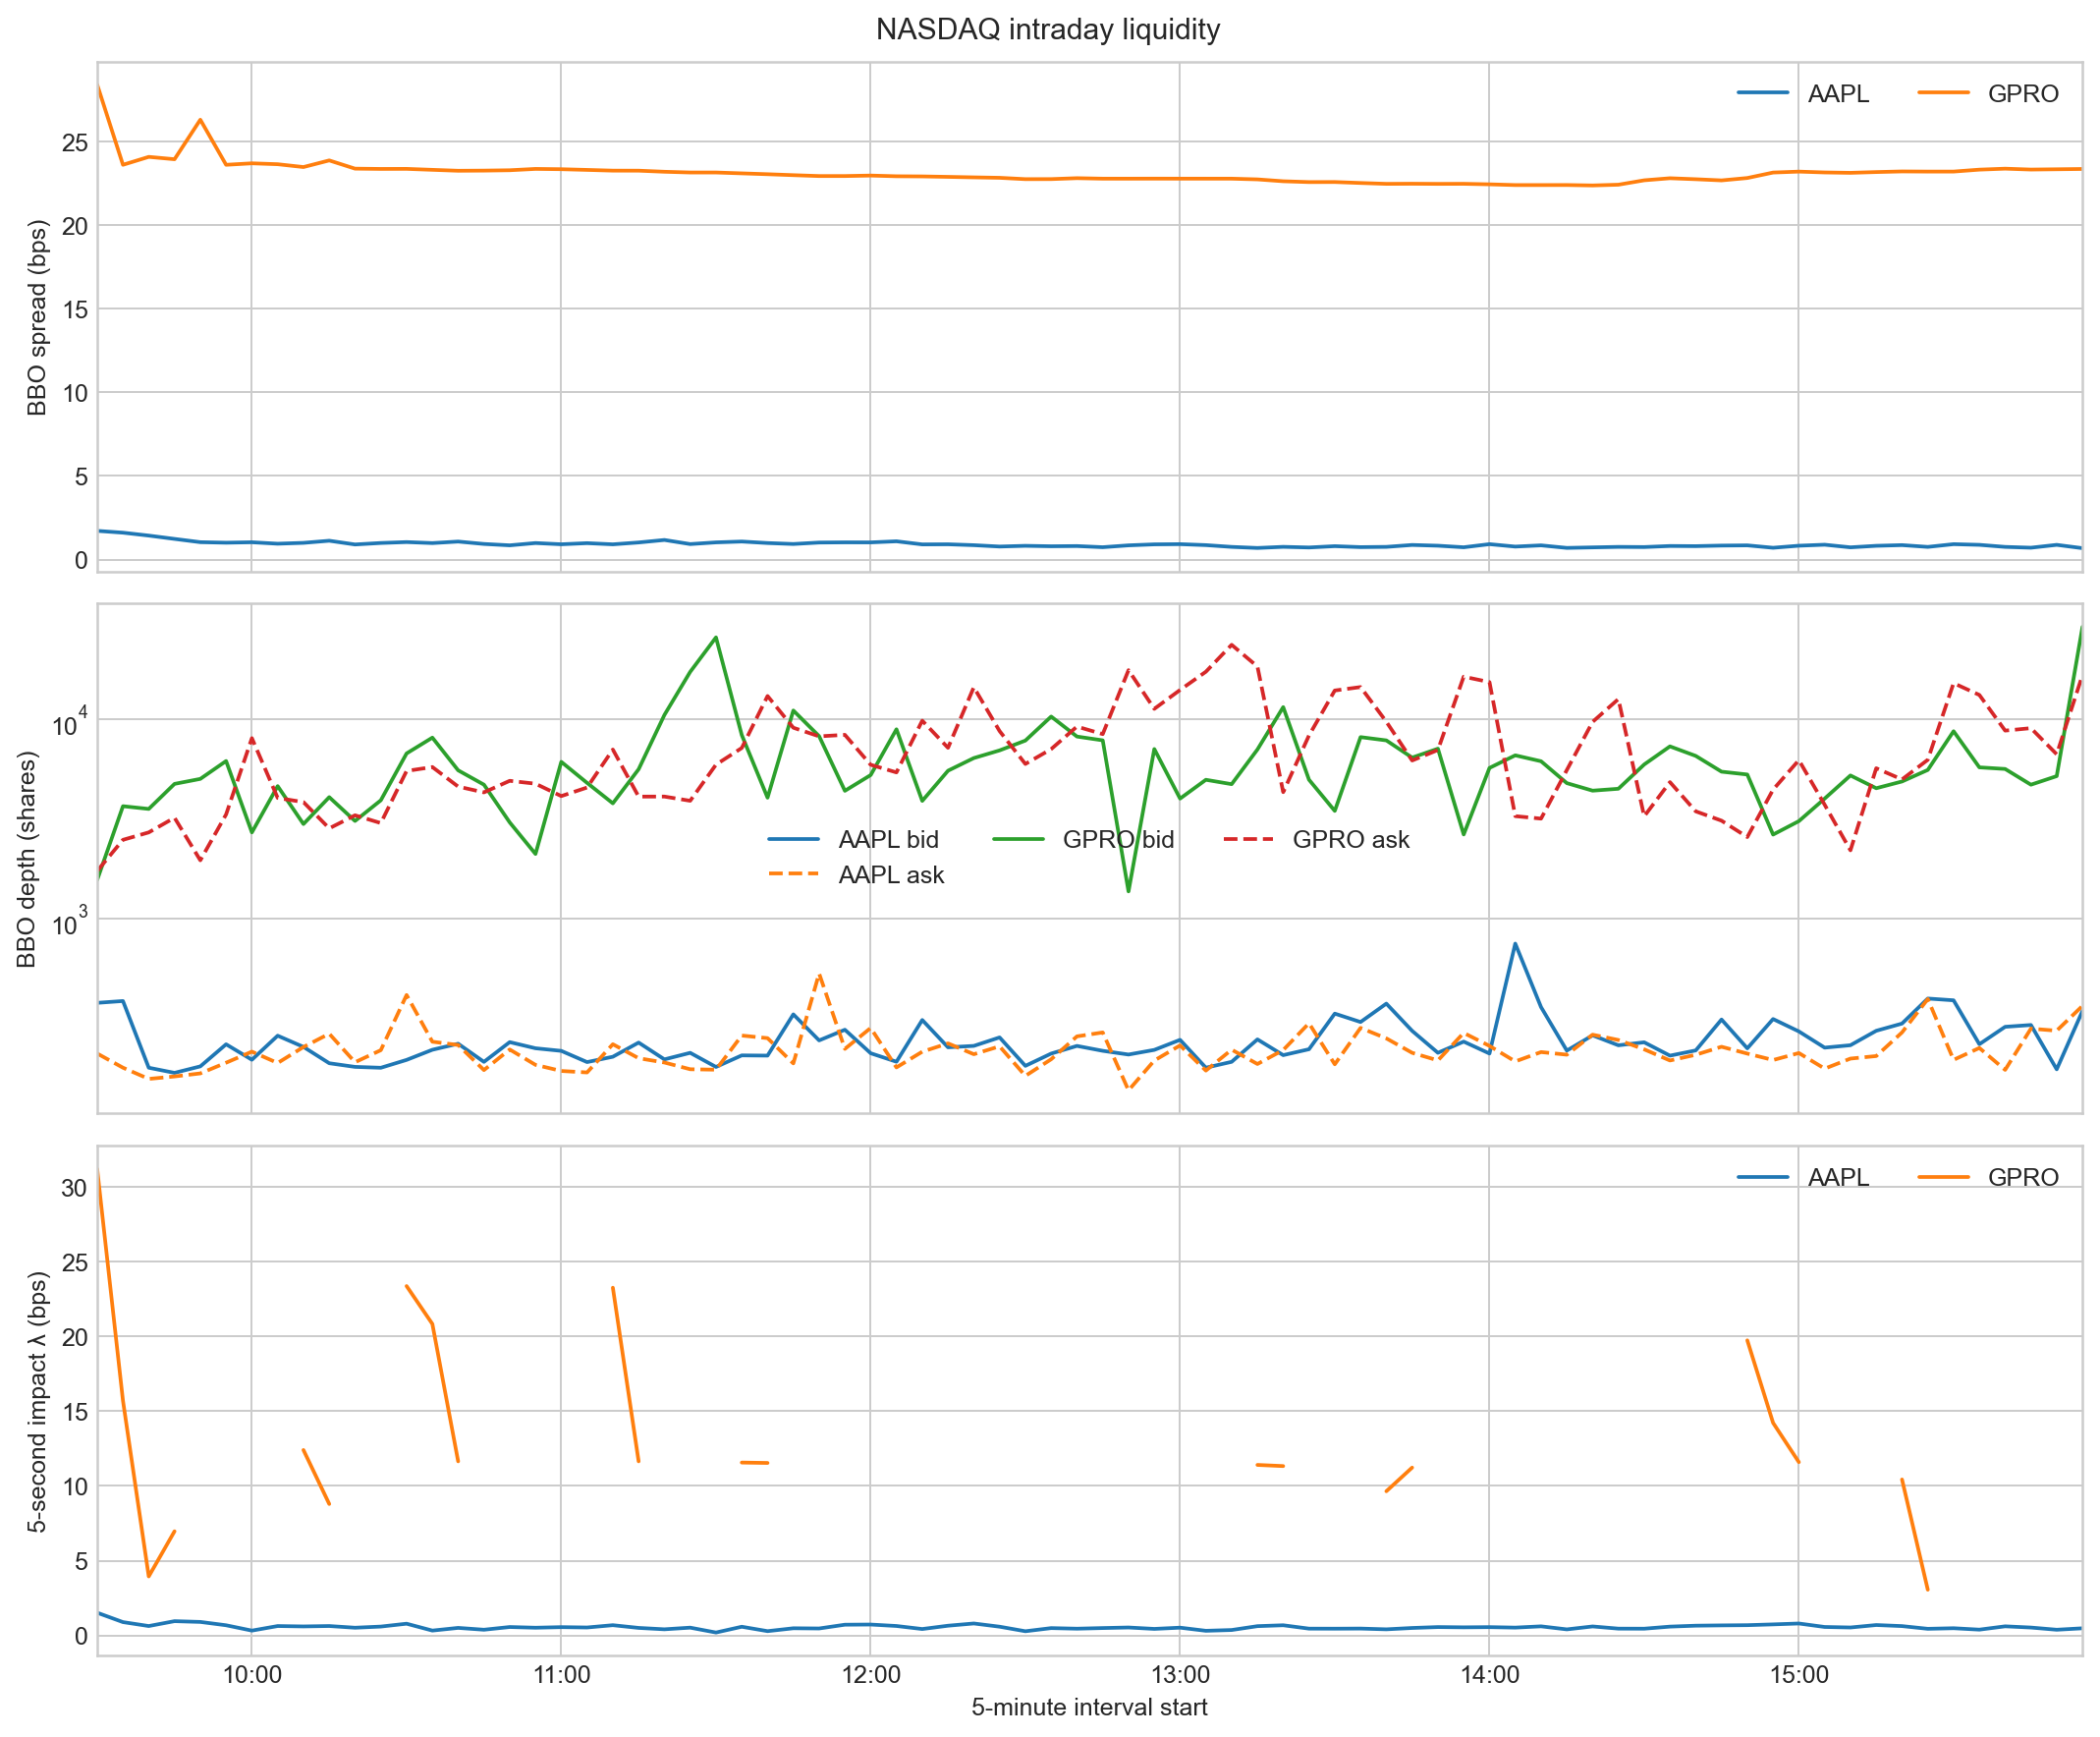
\includegraphics[width=\textwidth,height=0.84\textheight,keepaspectratio]{01_stock_liquidity_5min.png}
  \caption{NASDAQ five-minute liquidity. Spread and bid/ask depth are exact event-time-weighted means; impact is the mean of available minute-level signed-impact slopes. Spread is in basis points of five-minute VWAP.}
  \label{fig:stock-liquidity}
\end{figure}

\paragraph{Spread.}
Figure \ref{fig:stock-liquidity} shows that AAPL begins the session with a visibly wider spread, including a sharp disturbance around 09:45, and then settles toward roughly 0.8--1.0 basis points. Its mean opening-half-hour spread is \$0.0385, compared with \$0.0253 during the rest of the session. The late-day spread does not rebuild a second arm of a U-shape. On 30 December 2019, the Monday of a short New Year week, this is a day-specific holiday-week pattern rather than evidence against the usual intraday regularity.

GPRO behaves differently. Its spread is one cent at the 25th percentile, median, and 75th percentile, with a standard deviation of only 0.039 cents. On a \$4.34 stock, one cent is approximately 23 basis points. The nearly flat line is therefore not evidence of invariant information risk; it is evidence that the tick prevents further tightening.

\paragraph{Depth.}
Bid and ask depth cross repeatedly because the displayed imbalance changes sign. For AAPL, the touch is a small, continuously refreshed slice of a deeper multi-level book. GPRO displays more shares but less dollar value. This distinction explains why raw share depth should not be interpreted as greater economic liquidity. The $2\bar{s}$ statistics reinforce the point: the nearby book adds five to six times L1 for AAPL but only about twice L1 for GPRO.

\paragraph{Price impact.}
AAPL has an impact estimate in every minute and averages 0.56 basis points. Impact is 0.93 basis points during the first 30 minutes and 0.53 thereafter, consistent with faster information revelation and more expensive immediacy at the open. GPRO averages 13.25 basis points, but this mean is based on only 51 identified minutes. The median GPRO minute contains two trades, 105 minutes contain no trade, and a one-tick midquote movement is already about 23 basis points. Consequently, the disconnected GPRO line reflects both missing regressions and economically coarse, sparsely identified price moves. It should not be read as a continuously observed high-frequency signal.

\subsection{Foreign exchange}

\begin{figure}[p]
  \centering
  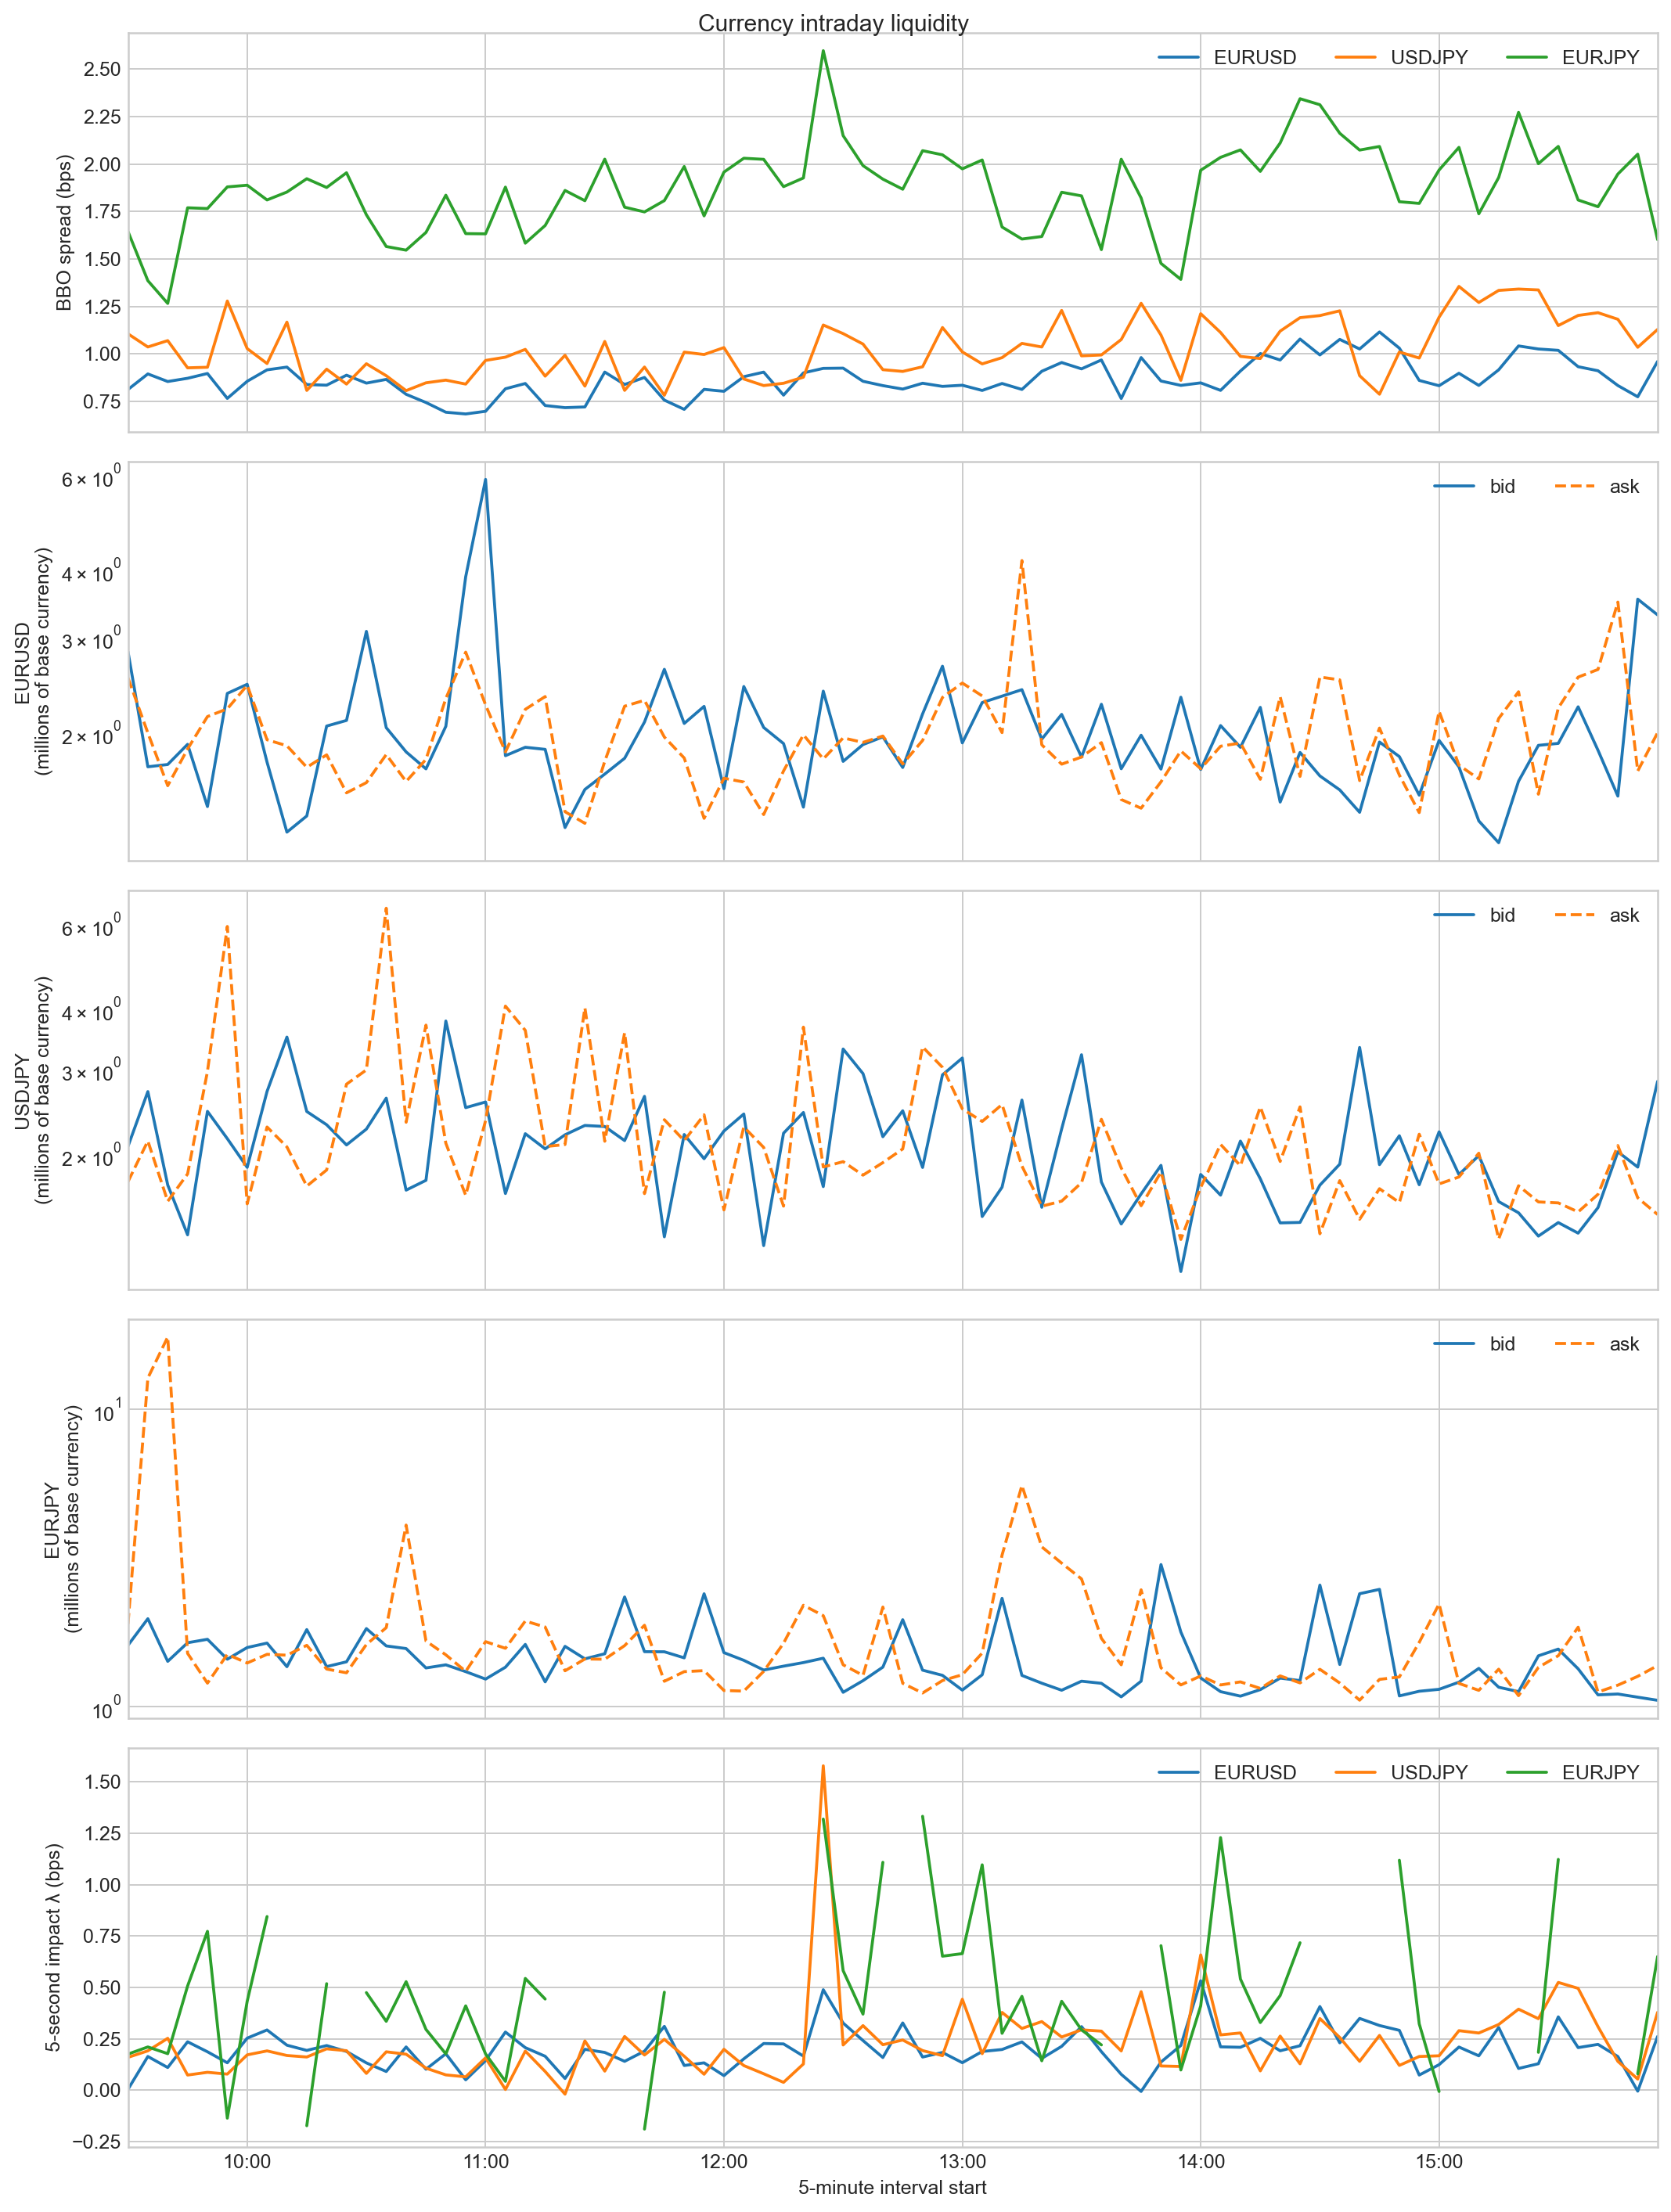
\includegraphics[width=\textwidth,height=0.90\textheight,keepaspectratio]{02_currency_liquidity_5min.png}
  \caption{Foreign-exchange five-minute liquidity. Depth is split by pair to keep bid/ask movements legible. The session clock is 09:30--16:00 on 25 January 2012.}
  \label{fig:fx-liquidity}
\end{figure}
\clearpage

\paragraph{Spread.}
The spread ranking is EUR/USD, USD/JPY, then EUR/JPY: approximately 0.87, 1.03, and 1.87 basis points. The cross is the synthetic residual of the two dollar legs and has the wider, sparser standalone book. All three remain far tighter than GPRO, while EUR/USD is comparable to AAPL in relative terms. The synchronized widening around 12:25---EUR/JPY reaches roughly 2.6 basis points---points to a common London-close event rather than three independent liquidity holes.

\paragraph{Depth.}
EUR/USD and USD/JPY generally display one to four million units at the touch. EUR/JPY is thinner, with median bid and ask depth near 1.3--1.4 million. The large EUR/JPY ask observation before 10:00 reaches nearly 49 million, but its 75th percentile is only 1.71 million; it is a short-lived posted order, not the typical state of the book. Roughly ten to eleven times L1 depth lies inside the $2\bar{s}$ band for all three pairs.

\paragraph{Price impact.}
EUR/USD is identified in 386 of 390 minutes and remains near 0.20 basis points. USD/JPY is identified in 302 minutes and experiences a pronounced impact spike at the same 12:25 time as the spread event. EUR/JPY resembles GPRO in data coverage, not in magnitude: it has 83 zero-trade minutes and only 103 impact estimates. Its mean identified impact is 0.46 basis points, more than twice EUR/USD. Impact is lower in the first 30 minutes than afterward for every currency pair, which is the opposite of AAPL and confirms that 09:30 New York is not the organizing event for this FX sample.

\section{Return Variation and Autocorrelation}

\begin{landscape}
\begin{table}[H]
\centering
\caption{Return diagnostics by sampling frequency}
\label{tab:return-diagnostics}
\scriptsize
\begin{threeparttable}
\begin{tabular}{@{}lllrrrrr@{}}
\toprule
Instrument & Frequency & Series & $N$ & Mean & Std. dev. & Realized variance & $\rho(1)$\\
\midrule
\multicolumn{8}{l}{\textit{Panel A: One-second log returns}}\\
AAPL & 1 second & Midquote & 23,399 & \num{3.302e-7} & \num{6.988e-5} & \num{1.143e-4} & 0.063\\
     &          & Transaction & 23,399 & \num{3.354e-7} & \num{7.348e-5} & \num{1.264e-4} & 0.037\\
GPRO & 1 second & Midquote & 23,399 & \num{5.001e-8} & \num{2.337e-4} & \num{1.278e-3} & 0.015\\
     &          & Transaction & 23,399 & \num{1.502e-7} & \num{2.103e-4} & \num{1.035e-3} & 0.072\\
EUR/USD & 1 second & Midquote & 23,399 & \num{4.602e-7} & \num{3.166e-5} & \num{2.345e-5} & 0.020\\
        &          & Transaction & 23,393 & \num{4.556e-7} & \num{3.537e-5} & \num{2.927e-5} & -0.021\\
USD/JPY & 1 second & Midquote & 23,399 & \num{-1.764e-7} & \num{2.542e-5} & \num{1.512e-5} & 0.035\\
        &          & Transaction & 23,391 & \num{-1.773e-7} & \num{3.001e-5} & \num{2.106e-5} & -0.013\\
EUR/JPY & 1 second & Midquote & 23,399 & \num{2.867e-7} & \num{3.077e-5} & \num{2.216e-5} & 0.046\\
        &          & Transaction & 23,340 & \num{2.855e-7} & \num{3.171e-5} & \num{2.347e-5} & 0.015\\
\addlinespace
\multicolumn{8}{l}{\textit{Panel B: One-minute log returns}}\\
AAPL & 1 minute & Midquote & 389 & \num{2.484e-5} & \num{5.715e-4} & \num{1.270e-4} & 0.105\\
     &          & Transaction & 389 & \num{2.497e-5} & \num{5.823e-4} & \num{1.318e-4} & 0.078\\
GPRO & 1 minute & Midquote & 389 & \num{-1.200e-5} & \num{1.880e-3} & \num{1.371e-3} & 0.015\\
     &          & Transaction & 389 & \num{-9.004e-6} & \num{1.802e-3} & \num{1.259e-3} & 0.044\\
EUR/USD & 1 minute & Midquote & 389 & \num{2.809e-5} & \num{2.712e-4} & \num{2.885e-5} & 0.011\\
        &          & Transaction & 389 & \num{2.799e-5} & \num{2.748e-4} & \num{2.960e-5} & -0.005\\
USD/JPY & 1 minute & Midquote & 389 & \num{-1.059e-5} & \num{2.695e-4} & \num{2.823e-5} & 0.004\\
        &          & Transaction & 389 & \num{-1.076e-5} & \num{2.739e-4} & \num{2.916e-5} & -0.003\\
EUR/JPY & 1 minute & Midquote & 389 & \num{1.743e-5} & \num{2.425e-4} & \num{2.294e-5} & -0.177\\
        &          & Transaction & 389 & \num{1.713e-5} & \num{2.481e-4} & \num{2.400e-5} & -0.149\\
\bottomrule
\end{tabular}
\begin{tablenotes}[flushleft]\footnotesize
\item \textit{Notes:} Returns are log differences of last-in-interval prices, with previous-tick carry-forward after the first valid observation. Realized variance is the unannualized sum of squared intraday returns. $\rho(1)$ is the full-session lag-1 sample autocorrelation.
\end{tablenotes}
\end{threeparttable}
\end{table}
\end{landscape}

Mean returns are small relative to their standard deviations. GPRO has substantially greater realized variance than AAPL at both horizons. Transaction-return variance is slightly above midquote variance for AAPL and the two dollar FX legs, consistent with bid--ask bounce. GPRO is the one-second exception: quote updates continue during seconds with no trade, so midquote realized variance exceeds transaction realized variance.

AAPL's one-minute midquote autocorrelation of $0.105$ indicates mild continuation rather than reversal. Its five-second impact is therefore not obviously undone at the next minute. GPRO's corresponding coefficient is only $0.015$, and the limited impact coverage prevents a strong permanence claim. EUR/JPY has one-minute transaction and midquote coefficients of $-0.149$ and $-0.177$, respectively, indicating temporary reversal on the thinner cross. EUR/USD and USD/JPY remain near zero, so this is not a general foreign-exchange finding.

\begin{figure}[H]
  \centering
  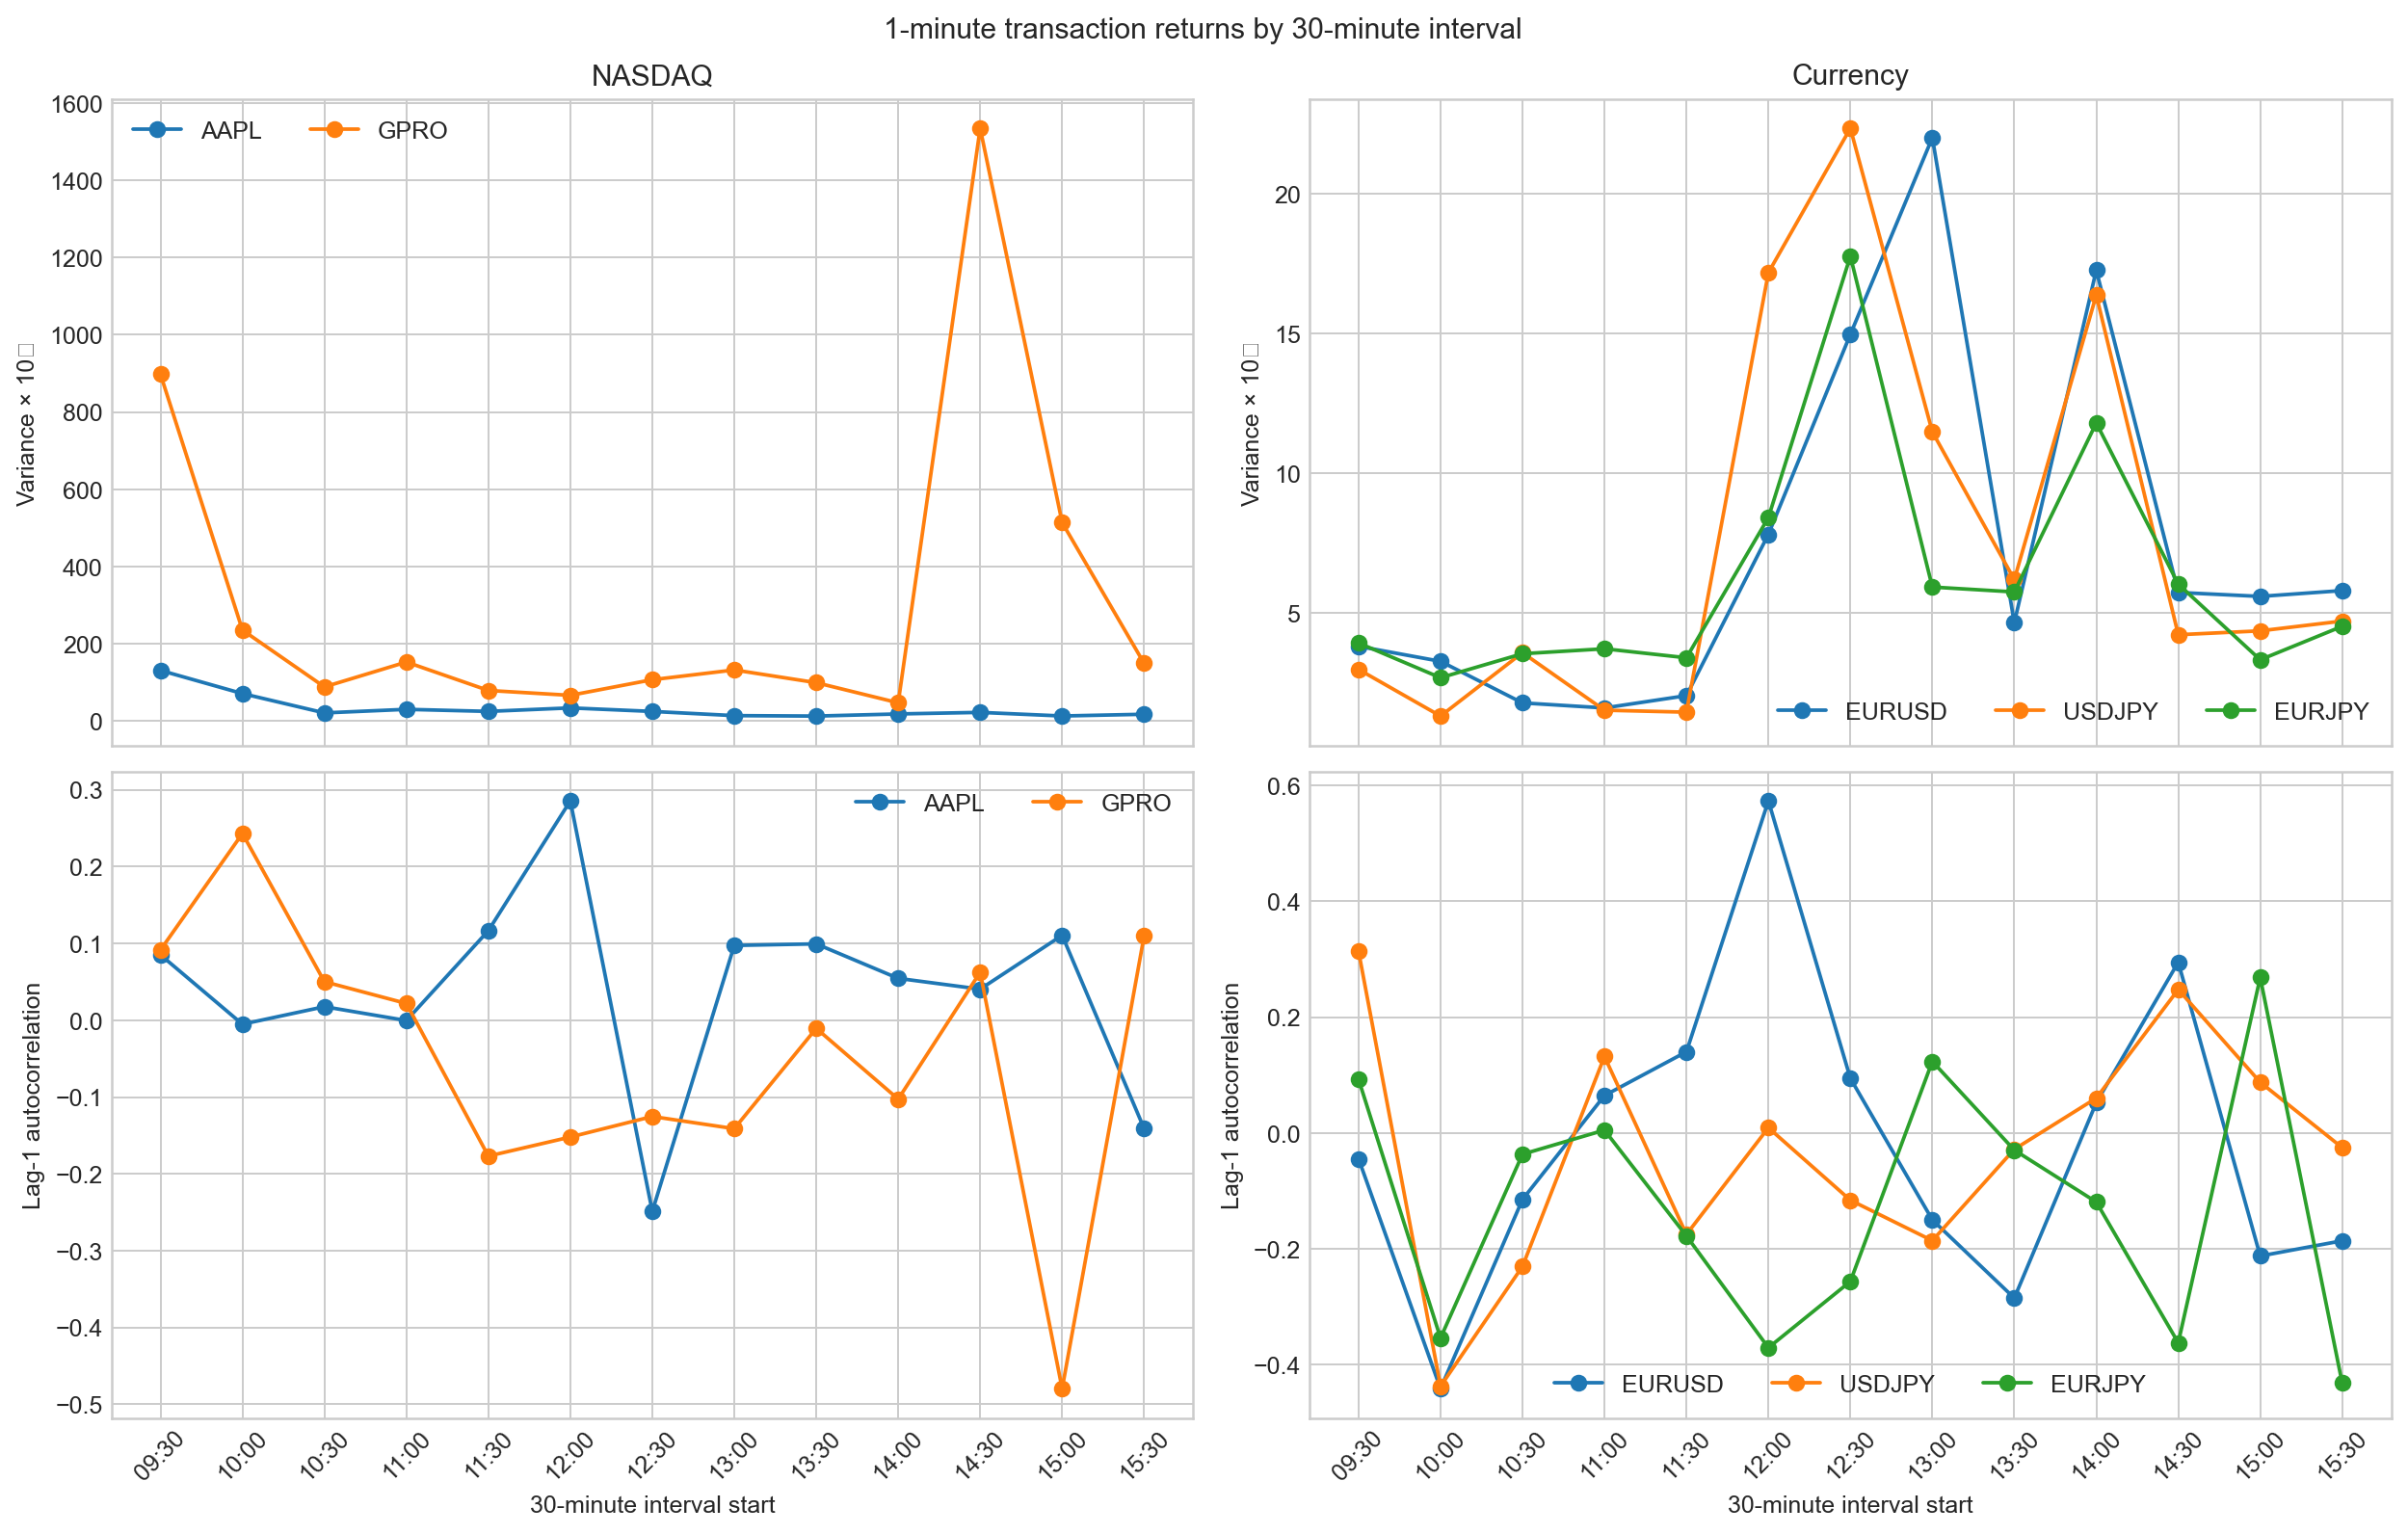
\includegraphics[width=\textwidth,height=0.80\textheight,keepaspectratio]{03_transaction_return_30min.png}
  \caption{Thirty-minute variance and lag-1 autocorrelation of one-minute transaction log returns.}
  \label{fig:variance-acf}
\end{figure}

\paragraph{AAPL versus GPRO variance.}
AAPL's opening-half-hour variance is \num{1.31e-6}; it then declines by approximately one order of magnitude and remains low. Lunch is near \num{1.3e-7}, and the final half-hour is \num{1.79e-7}. This path aligns with the wider opening spread and higher opening impact in Figure \ref{fig:stock-liquidity}, but not with a closing liquidity deterioration.

GPRO opens at \num{8.98e-6}, already about seven times AAPL's opening variance. Its largest observation is instead 14:30--15:00: \num{1.53e-5}, 32 times the preceding half-hour and about 67 times AAPL at the same clock time. The spread remains at one cent and bid depth rises rather than collapses, while the impact regression is unidentified around the event. The coherent interpretation is a sparse, one-sided transaction burst whose few large prints dominate a half-hour containing many carried-forward zero returns. The next bin remains volatile and has autocorrelation $-0.48$, indicating that much of the move is reversed rather than permanently incorporated.

\paragraph{Currency variance.}
All three currency pairs peak between 12:00 and 13:30. USD/JPY reaches \num{2.23e-7} at 12:30, EUR/USD reaches \num{2.20e-7} at 13:00, and EUR/JPY reaches \num{1.78e-7} at 12:30. This is the same interval as the common spread widening and USD/JPY impact spike. Depth does not collapse at the same time, so variance comoves more clearly with spread and impact than with L1 depth.

\paragraph{Thirty-minute autocorrelation.}
Each coefficient uses only 29 or 30 returns, giving an approximate standard error of $1/\sqrt{30}\simeq0.18$. Individual dots are therefore noisy. AAPL remains small throughout. GPRO's $-0.48$ coefficient at 15:00 is notable because it follows the 14:30 variance burst. Several EUR/JPY bins are materially negative, consistent with the full-session reversal in Table \ref{tab:return-diagnostics}. The isolated EUR/USD coefficient of $0.57$ at 12:00 is better read as temporary continuation into the London-close event than as stable predictability.

\begin{figure}[H]
  \centering
  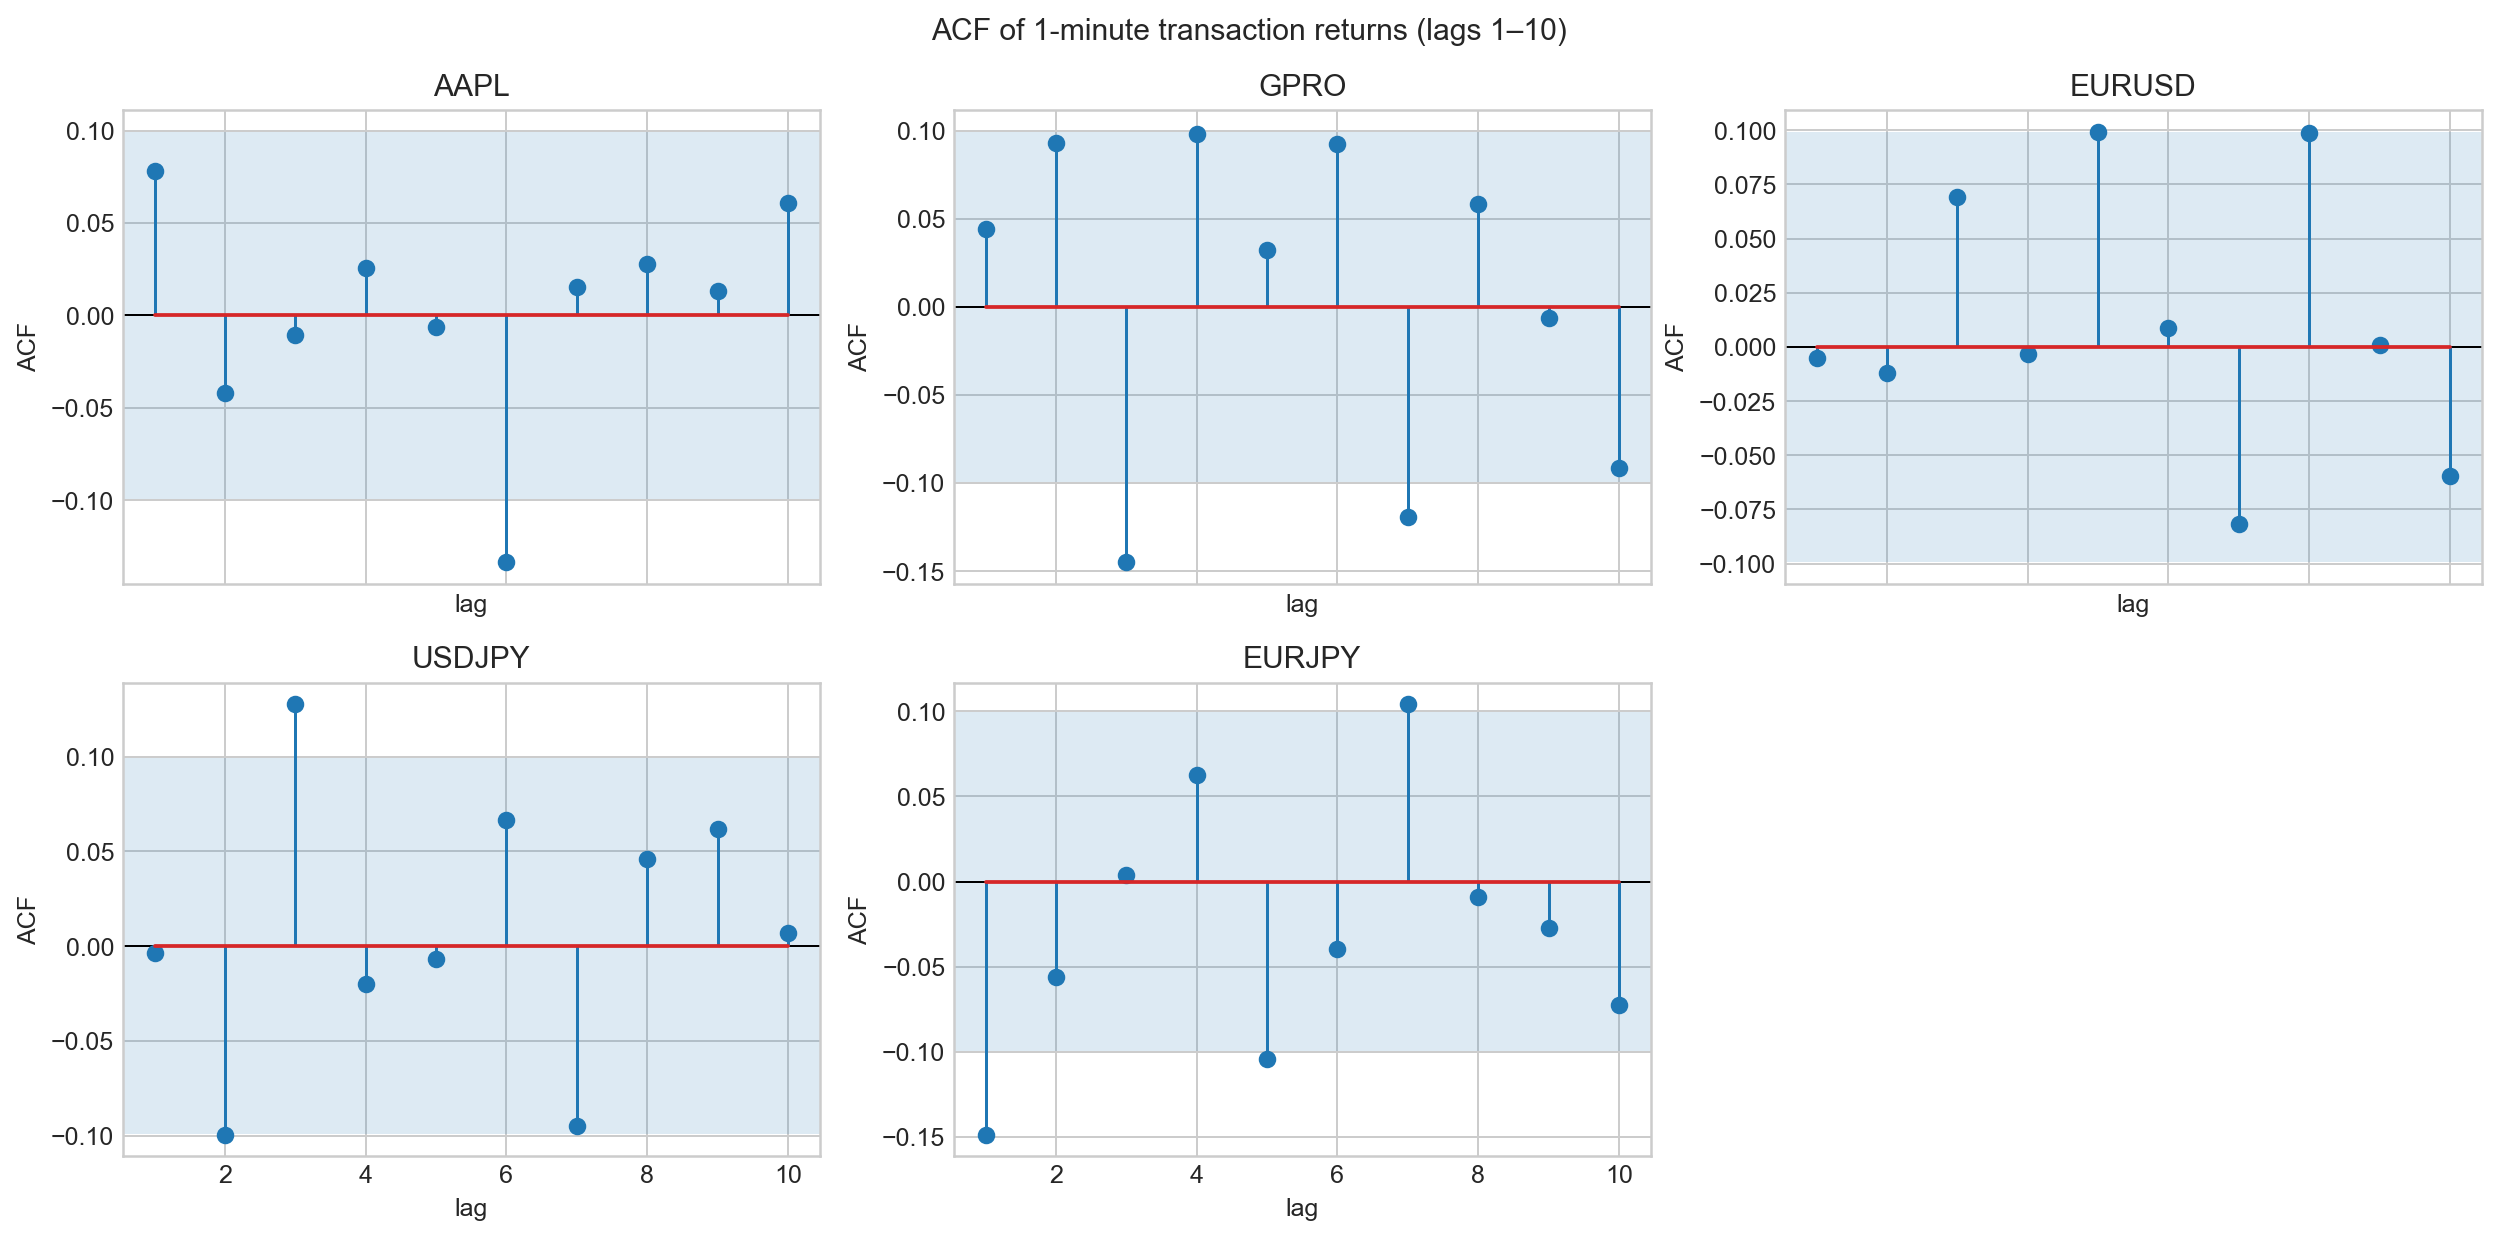
\includegraphics[width=\textwidth,height=0.75\textheight,keepaspectratio]{04_transaction_return_acf.png}
  \caption{Autocorrelation of one-minute transaction log returns, lags 1--10. The shaded band is $\pm1.96/\sqrt{T}$. Lag 0 is omitted.}
  \label{fig:acf}
\end{figure}

At lag 1, AAPL and GPRO are mildly positive but remain inside the full-sample noise band; EUR/USD and USD/JPY are effectively zero. EUR/JPY is the only lag-1 coefficient outside the band, at $-0.149$. Most dependence disappears by lags 2--3. The occasional later stem outside the band is isolated rather than persistent, so the ten-lag plot provides little evidence of a stable forecasting rule.

\section{Executable Triangular Arbitrage}

\begin{table}[H]
\centering
\caption{One-second triangular-arbitrage summary}
\label{tab:arb}
\small
\begin{threeparttable}
\begin{tabular}{@{}lr@{}}
\toprule
Statistic & Value\\
\midrule
Eligible seconds & 28\\
Fraction of 09:30--16:00 session & 0.120\%\\
Distinct episodes & 20\\
Mean episode duration & 1.4 seconds\\
Maximum episode duration & 6 seconds\\
Mean edge & 0.187 bps\\
Maximum edge & 1.181 bps\\
Mean binding quantity & 1.273 million EUR\\
Maximum binding quantity & 3.000 million EUR\\
Frictionless marked profit, all eligible seconds & \$678.14\\
\bottomrule
\end{tabular}
\begin{tablenotes}[flushleft]\footnotesize
\item \textit{Notes:} Every leg executes aggressively at the observed BBO. Twenty-five eligible seconds use Loop A and three use Loop B. Profit assumes full simultaneous execution at the displayed size and excludes all trading frictions.
\end{tablenotes}
\end{threeparttable}
\end{table}

\subsection{A six-second episode}

The longest episode begins at 09:36:35. In each of six consecutive seconds, Loop A sells euros for dollars at the EUR/USD bid, sells the dollars for yen at the USD/JPY bid, and buys the euros back at the EUR/JPY ask. The loop product is $1.00000397037$, or 0.040 basis points. Binding size is EUR 2 million for the first three seconds and EUR 3 million for the last three. Full execution every second would mark approximately \$77 before costs. Loop B remains below one throughout, so the result is one-sided rather than a crossed-book artifact.

The economically largest observation occurs at 09:43:32. Loop A widens from 0.18 to 0.49 and then 1.18 basis points over three seconds, with a binding size near EUR 771 thousand. The peak second marks about \$118 and disappears one second later.

Across the day, the 28 eligible seconds cluster in two windows, 09:34--09:43 and 13:15--14:18. The afternoon cluster overlaps the tail of the London-close variance event and its 14:00 aftershock, but the clocks are not identical. Almost all observations use Loop A.

\subsection{Economic feasibility}

The \$678 total is an upper bound, not cash that was necessarily available. The six-second episode is persistent but only 0.04 basis points wide, equivalent to \$10--\$15 per second at the displayed quantity. A last-look rejection, one-second delay, brokerage charge, or partial fill can remove the gain. The 1.18-basis-point observation is more attractive but lasts only one second. Since the files do not reveal exchange-to-user latency, firm-quote status, fees, or simultaneous fill probabilities, the evidence establishes apparent executable BBO triangles in historical data, not a deployable live strategy.

\section{Conclusion}

The cross-sectional results are consistent with liquidity and information-asymmetry theory. The less active GPRO book carries a much larger relative spread and signed price impact than AAPL. However, the mechanism matters: GPRO's quoted spread is pinned by the tick, and raw share depth exaggerates its economic liquidity. AAPL's opening spread, impact, and variance move together, while its close remains quiet on this particular holiday-week session.

Foreign exchange follows a different clock. The London close produces the dominant spread, impact, and variance event, and EUR/JPY is persistently the widest and sparsest leg. Its negative one-minute autocorrelation indicates temporary reversal rather than a permanent common FX pattern. Triangular-arbitrage observations occur in the same broad afternoon window but are rare, short, and economically fragile.

The report therefore supports the standard theory only as far as the tape allows: greater relative illiquidity is associated with greater impact, but intraday shapes depend on tick constraints, trading intensity, market-specific clocks, and the finite identification available in one day of data. The Monday--Friday extension remains necessary to determine which shapes are persistent and which are specific to the selected sessions; the weekly implications stated in Section \ref{sec:week} should be treated as testable hypotheses rather than as additional findings.

\appendix
\section{Function Timing Versus Opportunity Duration}

\begin{table}[H]
\centering
\caption{Wall-clock timing of the locked notebook run}
\label{tab:timing}
\small
\begin{threeparttable}
\begin{tabular}{@{}lr@{}}
\toprule
Pipeline step & Seconds\\
\midrule
Load and reconstruct NASDAQ books & 136.022\\
Load and reconstruct currency books & 316.155\\
Compute per-minute statistics & 1.228\\
Construct price series, returns, and ACFs & 0.648\\
Compute 30-minute diagnostics & 0.291\\
Detect triangular arbitrage & 0.529\\
Plot NASDAQ liquidity & 8.221\\
Plot currency liquidity & 9.479\\
Plot 30-minute variance and ACF & 5.434\\
Plot full-sample ACF & 3.392\\
\midrule
Total timed wall clock & 481.399\\
\bottomrule
\end{tabular}
\begin{tablenotes}[flushleft]\footnotesize
\item \textit{Notes:} Timings are from the final notebook outputs and depend on hardware, local file access, and software state. Detection is timed after the synchronized one-second books already exist in memory.
\end{tablenotes}
\end{threeparttable}
\end{table}

The arbitrage scan takes 0.529 seconds once the books are built, compared with a mean episode length of 1.4 seconds and a maximum of 6 seconds. Thus, the vectorized historical detector is faster than the mean observed window. That comparison does not imply live feasibility. The 452 seconds spent loading and reconstructing historical books are an offline research cost, not the latency of an incremental feed handler. Conversely, a live system must receive three quotes, update three books, test both loops, route three aggressive orders, and obtain simultaneous fills before the opportunity closes. The present timing table measures only the Python research pipeline and cannot measure that end-to-end trading clock.

\begin{thebibliography}{9}

\bibitem{glosten1985}
Lawrence R. Glosten and Paul R. Milgrom.
\newblock Bid, ask and transaction prices in a specialist market with heterogeneously informed traders.
\newblock \emph{Journal of Financial Economics}, 14(1):71--100, 1985.

\bibitem{kyle1985}
Albert S. Kyle.
\newblock Continuous auctions and insider trading.
\newblock \emph{Econometrica}, 53(6):1315--1335, 1985.

\end{thebibliography}

\end{document}
